\documentclass[12pt]{article}
% \usepackage{polski}
\usepackage[utf8]{inputenc}

\usepackage{lingmacros}
\usepackage{tree-dvips}
\usepackage{blindtext}
\usepackage{graphicx}
\graphicspath{ {imgs/} }


\setcounter{secnumdepth}{0}
\pagenumbering{gobble}

% \usepackage[top=0.1in, bottom=0.7in, left=1.35in, right=1.35in]{geometry}

\title{Lifelong Learning With Dynamically Expandable Networks -- Reproducibility Report }
\author{Błażej Sowa, Łukasz Siudek}
\date{}

\begin{document}
\maketitle

\section {Motivation}

Lifelong learning (Thrun, 1995), the problem of continual learning where tasks arrive in sequence, is
an important topic in transfer learning. The primary goal of lifelong learning is to leverage knowledge
from earlier tasks for obtaining better performance, or faster convergence/training speed on models
for later tasks. While there exist many different approaches to tackle this problem, we consider
lifelong learning under deep learning to exploit the power of deep neural networks. Fortunately, for
deep learning, storing and transferring knowledge can be done in a straightforward manner through
the learned network weights. The learned weights can serve as the knowledge for the existing tasks,
and the new task can leverage this by simply sharing these weights.

\section {Reproducibility}

\subsection {Subsection 1}
This is a subsection.

\subsection {Subsection 2}

The following image does not show any wombats
\includegraphics[height=\baselineskip]{example-image}.
  
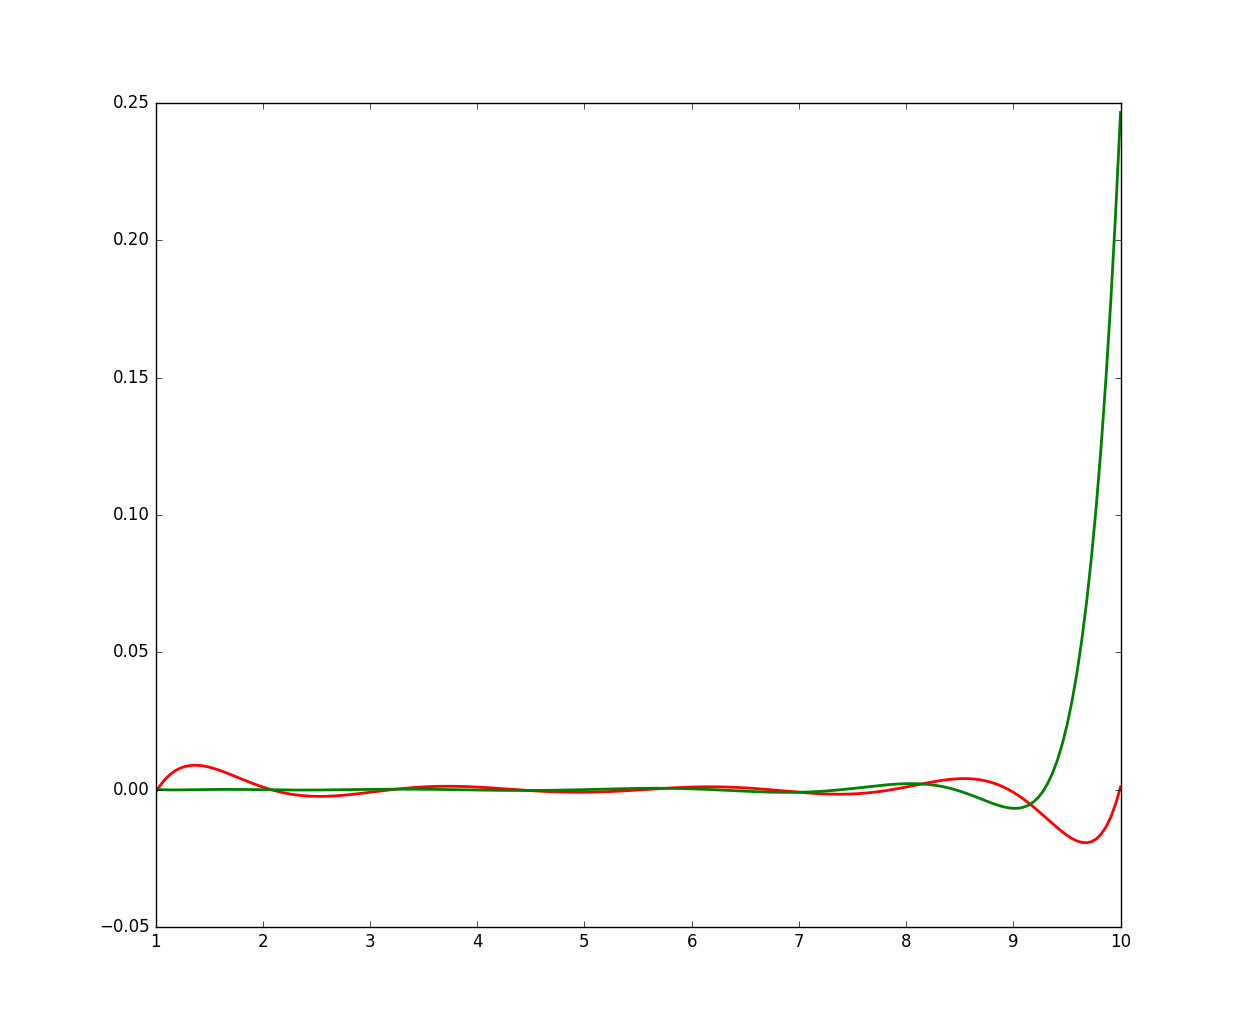
\includegraphics[height=3cm]{figure_1.png}

\includegraphics[height=3cm]{example-image-a} \includegraphics[width=5cm]{example-image-b}

\section {Conclusion}

Conclusion.

% Zawartość sceny do wyrenderowania znajduje się w pliku \texttt{scene.ml}.

\begin{thebibliography}{9}
    \bibitem{lamport94}
        Leslie Lamport,
        \textit{\LaTeX: a document preparation system},
        Addison Wesley, Massachusetts,
        2nd edition,
        1994.
\end{thebibliography}

\end{document}
    